\documentclass[12pt]{article}
\usepackage[a4paper, total={6in, 9in}]{geometry}
\usepackage[utf8]{inputenc}
\usepackage[T1]{fontenc}
\usepackage{lmodern}
\usepackage{graphicx}
\usepackage{float}
\usepackage{csquotes}
\usepackage{lipsum}
\usepackage{enumitem}
\usepackage{xcolor}
\usepackage{booktabs}
\usepackage{adjustbox}
\usepackage{listings}
\usepackage{caption}
\usepackage{hyperref}
\usepackage{listings}
\usepackage{tcolorbox}
\usepackage{seqsplit}

\renewcommand{\figurename}{Figura}
\hypersetup{colorlinks=true, urlcolor=blue}

\tcbuselibrary{listingsutf8}
\newtcblisting{terminal}{
    listing only,
    listing options={
        basicstyle=\ttfamily\color{white}\small,
        backgroundcolor=\color{black},
        keywordstyle=\color{cyan},
        commentstyle=\color{green},
        identifierstyle=\color{white},
        language=bash,
        breaklines=true,
        showstringspaces=false,
        numbers=none,
        deletekeywords={do},
    },
    colframe=black,
    colback=black,
    sharp corners,
    boxsep=1mm,
    left=2mm,
    right=2mm,
    top=1mm,
    bottom=1mm,
}

\lstdefinestyle{vscode}{
    language=Java,
    extendedchars=true,
    inputencoding=ansinew,
    tabsize=4,
    showstringspaces=false,
    numbers=left,
    firstnumber=1,
    commentstyle=\color{gray},        
    keywordstyle=\color{blue},        
    stringstyle=\color{orange},
    rulecolor=\color{black},
    basicstyle=\small\ttfamily,
    breaklines=true,
    numberstyle=\tiny,
    aboveskip=1em,
    belowskip=1em,
}

\lstdefinestyle{json}{
    belowcaptionskip=1\baselineskip,
    breaklines=true,
    frame=false,
    xleftmargin=\parindent,
    language=Java,
    showstringspaces=false,
    basicstyle=\footnotesize\ttfamily,
    keywordstyle=\bfseries\color{green!40!black},
    commentstyle=\itshape\color{purple!40!black},
    stringstyle=\color{orange},
    numbers=left,
    numbersep=5pt,
    numberstyle=\tiny\color{gray},
    backgroundcolor=\color{gray!10},
    tabsize=2
}

\graphicspath{{./images/}}

\title{\textbf{Sistema Extensível de Gestão de Dados Mestres}}
\date{Engenharia de Software II}
\author{Bruno Laitano, Daniel Lee e Pedro Dorneles}

\begin{document}

\maketitle

\section{Introdução}
Com uma arquitetura de integração eficiente, extensível e flexível, desenvolvemos um sistema \emph{Master Data Management} capaz de consolidar, padronizar e garantir a qualidade e a governança de dados mestres provenientes da API pública \href{https://restcountries.com/v3.1/all}{\emph{REST Countries}}, com dezenas de dados geográficos a respeito de 250 países do globo.

\quad Para tanto, idealizamos dois serviços distintos: o \emph{Master Data Management} (MDM) e o \emph{Data Extraction Management} (DEM). O MDM é responsável por armazenar, validar e padronizar os dados mestres. Ele provê uma API \emph{RESTful} própria que permite operações administrativas sobre os registros, possibilitando a criação de novos dados, a recuperação de informações com base em critérios específicos, a atualização de registros existentes e a exclusão de dados obsoletos ou redundantes, mantendo um repositório central confiável e estruturado.

\quad Por outro lado, o DEM tem como função principal executar operações de ETL (Extração, Transformação e Carga) a partir da API \emph{REST Countries}. Esse serviço realiza a extração dos dados geográficos, aplica transformações para padronizar as informações conforme critérios pré-definidos e, em seguida, carrega os dados transformados em um arquivo \texttt{.json}. Além disso, disponibiliza APIs \emph{RESTful} próprias que permitem não apenas monitorar as transações realizadas, mas também expondo ao outro serviço a nova coleção de dados baseada na original.

\quad Do ponto de vista arquitetural, utilizamos H2 e JPA para estruturar o nosso projeto. O H2 é um banco de dados relacional capaz de facilitar a configuração e o \emph{reset} do ambiente a cada execução. Já o JPA é uma especificação para mapeamento objeto-relacional, permitindo que entidades Java sejam persistidas e consultadas no banco de dados, sem a necessidade de escrever comando SQL manualmente.

\section{\emph{Data Extraction Management}}
O serviço extrator é baseado na extração dos dados "crus" (\texttt{raw}) da API \emph{REST Countries}, na transformação desses dados em uma nova coleção, com menos atributos, e no registro local dos dados curados (\texttt{bronze}). Além disso, um segmento específico do serviço é dedicado a preparar metadados a respeito das informações coletadas durante a extração.

\subsection{ETL: \emph{Extract, Transform, Load}}
A leitura da API pública é realizada com \texttt{RestTemplate}, que fornece dezenas de operações abrangendo todos os parâmetros de requisição HTTP. Essa estrutura é especialmente utilizada no contexto de uma classe \texttt{ExtractService}.

\quad O serviço de extração, além de consumir a API, registra uma cópia local em formato \texttt{.json} dos dados geográficos coletados. Isso é realizado por meio de uma operação \texttt{saveRaw()}, que nomeia cada arquivo coletado a partir do tempo e da data de extração, garantindo que os registros locais possam ser mapeados em função do momento em que foram extraídos.

\quad Uma vez extraídos, os dados "crus" são transformados com base em atributos previamente selecionados. A transformação se dá sobre duas entidades: \texttt{Country} e \texttt{Currency}, sendo esta última uma propriedade específica da primeira. Do ponto de vista do banco de dados, ambas estão interrelacionadas por meio de um par chave primária (\texttt{PK})/chave estrangeira (\texttt{FK}).

\begin{figure}[H]
\centering
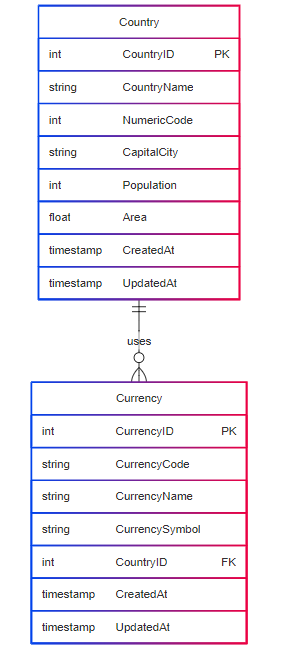
\includegraphics[scale=0.5]{assets/Diagram.png}
\caption{Esquema original na requisição do projeto}
\end{figure}

\quad Foram adicionados ao esquema de \texttt{Country} novos atributos em relação à proposta original. Abaixo, você poderá ver, no contexto da classe/entidade dedicada à figura do país, quais foram as propriedades incluídas no design. Os atributos de \texttt{Currency} foram mantidos como o exigido no esquema original. Além disso, atribuímos a cada objeto um identificador único utilizando a classe \texttt{UUID}.

\begin{lstlisting}[style=vscode]
public class Country {
    private String id;
    private String commonName;
    private Boolean independent;
    private Boolean unMember;
    private List<Currency> currencies;
    private String capital;
    private String region;
    private String languages;
    private String latlng;
    private String borders;
    private Double area;
    private Long population;
    private String gini;
    private String timezones;
    private String continents;
    @JsonFormat(shape = JsonFormat.Shape.STRING, pattern = "yyyy-MM-dd'T'HH:mm:ss")
    private Timestamp createdAt;
    @JsonFormat(shape = JsonFormat.Shape.STRING, pattern = "yyyy-MM-dd'T'HH:mm:ss")
    private Timestamp updatedAt;
}
\end{lstlisting}

\quad As informações curadas são salvas localmente em um arquivo no formato \texttt{.json}, também nomeado a partir do momento do registro, por meio de uma operação \texttt{saveBronze()}. Os arquivos curados são classificados como \texttt{bronze}. A ideia de nomeá-los de tal forma deve-se ao fato de que, na hipótese de novos refatoramentos das informações a serem coletadas, os dados podem ser transformados de forma cada vez mais precisa (\texttt{silver}, \texttt{gold}...).

\quad Finalmente, um \texttt{DemController} expõe uma nova API ao outro serviço que compõe este projeto, garantindo que os dados transformados também possam ser acessados livremente. Abaixo, indicamos a função do tipo \texttt{@GetMapping} responsável por publicizar essas informações.

\begin{lstlisting}[style=vscode]
@GetMapping("")
    public ResponseEntity<String> getCountries() {
        String bronzeData = data.getBronzeData();
        if (bronzeData == null) {
            return ResponseEntity.status(HttpStatus.NOT_FOUND)
                    .contentType(MediaType.APPLICATION_JSON)
                    .body("{\"error\":\"No bronze data available.\"}");
        }
        return ResponseEntity.ok()
                .contentType(MediaType.APPLICATION_JSON)
                .body(bronzeData);
    }
\end{lstlisting}

\subsection{Metadados}
Os metadados a respeito de cada extração são salvos com base em três parâmetros: o nome da fonte (\texttt{provider}), a quantidade de elementos salvos (\texttt{count}) e a última atualização recebida (\texttt{lastUpdate}). Criamos tanto um repositório quanto um controlador para que os metadados possam ser registrados localmente e expostos em um novo \emph{endpoint}.

\quad A título de exemplo, realizada uma extração, é este o tipo de resultado que poderá ser conferido pelo administrador:

\begin{lstlisting}[style=json]
[
    {
        "provider": "RestCountries API",
        "count": 250,
        "lastUpdate": "2025-05-25_12-19-10"
    }
]
\end{lstlisting}

\section{\emph{Master Data Management}}
O módulo MDM foi desenvolvido com o objetivo de gerenciar dados mestres relacionados a países e moedas, proporcionando operações de criação, consulta, atualização e remoção através de uma API \emph{RESTful} implementada com \emph{Spring Boot}. A seguir, são descritas as principais classes que compõem esse módulo.

\subsection{\texttt{CountryController}}
O \texttt{CountryController} provê a API \emph{RESTful} para o gerenciamento das entidades de país (\texttt{CountryEntity}), cumprindo diretamente os requisitos de criação, consulta, atualização e remoção definidos na especificação do microserviço MDM.

\begin{table}[H]
\centering
\caption{Endpoints da classe \texttt{CountryController}}
\begin{adjustbox}{max width=\textwidth}
\begin{tabular}{@{} l c p{8cm} @{}}
\toprule
\textbf{Endpoint} & \textbf{Método HTTP} & \textbf{Descrição} \\
\midrule
\texttt{/mdm/countries/all} & GET & Retorna a lista completa de países cadastrados, via \texttt{CountryService.getAll()} \\
\texttt{/mdm/countries/id/\{id\}} & GET & Busca país por identificador UUID, retornando \texttt{200 OK} ou \texttt{404 Not Found} \\
\texttt{/mdm/countries/name/\{name\}} & GET & Busca país pelo nome comum (\texttt{commonName}), retornando \texttt{200 OK} ou \texttt{404 Not Found} \\
\texttt{/mdm/countries/capital/\{capital\}} & GET & Busca país pela capital \\
\texttt{/mdm/countries/region/\{region\}} & GET & Filtra países por região \\
\texttt{/mdm/countries/borders/\{border\}} & GET & Retorna todos os países que fazem fronteira com o código ISO especificado \\
\texttt{/mdm/countries/create} & POST & Cria um novo registro de país, recebendo JSON com todos os atributos de \texttt{CountryEntity} \\
\texttt{/mdm/countries/update/\{id\}} & PATCH & Atualiza parcialmente um país existente, através de um \texttt{Map<String,Object>} de campos \\
\texttt{/mdm/countries/delete/\{id\}} & DELETE & Remove o país identificado por \texttt{id} \\
\bottomrule
\end{tabular}
\end{adjustbox}
\end{table}

\subsubsection{Detalhes de implementação}
\begin{itemize}
    \item \textbf{Injeção de dependências}: o controlador recebe via construtor o \texttt{CountryService}, responsável pela lógica de negócio, e o \texttt{CountryRepository}, que executa operações de persistência;
    
    \item \textbf{Tratamento de respostas}: métodos que retornam um \texttt{Optional} são encapsulados com \texttt{ResponseEntity}, garantindo retornos apropriados como \texttt{200 OK} ou \texttt{404 Not Found};
    
    \item \textbf{Consultas personalizadas}: filtros por região e fronteiras são implementados utilizando \texttt{Stream API} sobre a lista completa de países.
\end{itemize}

\subsubsection{Exemplo de \emph{payload} para a criação de um novo país}
\texttt{POST /mdm/countries/create}

\begin{lstlisting}[style=json]
{
  "id": "b3f5c8e2-9f1e-4a7a-8d8f-2a4e5c6d7b8c",
  "commonName": "Brazil",
  "independent": true,
  "unMember": true,
  "currencies": [
    {
      "id": "e2f1a9d8-3b4c-5e6f-7a8b-9c0d1e2f3a4b",
      "currencyCode": "BRL",
      "name": "Brazilian real",
      "symbol": "R$"
    }
  ],
  "capital": "Brasilia",
  "region": "Americas",
  "languages": "Portuguese",
  "latlng": "[-15.793889, -47.882778]",
  "borders": ["ARG","BOL","COL","GUF","GUY","PRY","PER","SUR","URY","VEN"],
  "area": 8515767.0,
  "population": 212559409,
  "gini": "53.4",
  "timezones": ["UTC-05:00","UTC-04:00","UTC-03:00"],
  "continents": ["South America"]
}
\end{lstlisting}

\subsubsection{Exemplo de \emph{payload} para atualização parcial}
\texttt{PATCH /mdm/countries/update/b3f5c8e2-9f1e-4a7a-8d8f-2a4e5c6d7b8c}

\begin{lstlisting}[style=json]
{
  "population": 213000000,
  "gini": "54.7"
}
\end{lstlisting}

\subsection{\texttt{CurrencyController}}
O \texttt{CurrencyController} fornece a API \emph{RESTful} para o gerenciamento de moedas (\texttt{CurrencyEntity}), completando o escopo de domínio financeiro do MDM.

\begin{table}[H]
\centering
\caption{Endpoints da classe \texttt{CurrencyController}}
\begin{adjustbox}{max width=\textwidth}
\begin{tabular}{@{} l c p{8cm} @{}}
\toprule
\textbf{Endpoint} & \textbf{Método HTTP} & \textbf{Descrição} \\
\midrule
\texttt{/mdm/currencies/all} & GET & Lista todas as moedas disponíveis no repositório \\
\texttt{/mdm/currencies/id/\{id\}} & GET & Retorna moeda por UUID, com \texttt{200 OK} ou \texttt{404 Not Found} \\
\texttt{/mdm/currencies/code/\{code\}} & GET & Busca moeda pelo código ISO (e.g. \texttt{"USD"}), retornando um \texttt{Optional<CurrencyEntity>} \\
\texttt{/mdm/currencies/create} & POST & Cria uma nova moeda, recebendo JSON com atributos de \texttt{CurrencyEntity} \\
\texttt{/mdm/currencies/update/\{id\}} & PATCH & Atualiza parcialmente uma moeda existente \\
\texttt{/mdm/currencies/delete/\{id\}} & DELETE & Remove a moeda pelo identificador \\
\bottomrule
\end{tabular}
\end{adjustbox}
\end{table}

\subsubsection{Detalhes de implementação}
\begin{itemize}
    \item \textbf{Consultas}: busca por código de moeda (\texttt{getByCode}) retornando \texttt{Optional}, permitindo tratamento seguro de resultados;
    
    \item \textbf{Responsabilidade}: validação de formatos (ISO 4217) e regras de negócio são realizadas na camada de serviço (\texttt{CurrencyService});
    
    \item \textbf{Padrão \emph{RESTful}}: todos os métodos seguem boas práticas REST, garantindo consistência com demais serviços.
\end{itemize}

\subsubsection{Exemplo de \emph{payload} para criação de uma nova \emph{currency}}
\texttt{POST /mdm/currencies/create}

\begin{lstlisting}[style=json]
{
    "currencyCode": "FCR",
    "currencyName": "Fictional currency",
    "currencySymbol": "Fcr"
}
\end{lstlisting}

\section{Integração entre DEM e MDM}
A forma como definimos a integração entre ambos os serviços implementados envolve dois segmentos criados no contexto de MDM. Em \texttt{CountryService}, um método com a anotação \texttt{@PostConstruct}, sendo executado logo após a conclusão da injeção de dependências, é responsável por permitir o acesso de MDM aos dados transformados (\texttt{bronze}) em DEM. O método foi chamado de \texttt{syncWithDem()}.

\quad A razão pela qual optamos por permitir ao MDM acessar os dados transformados é que, dessa forma, as operações \texttt{CRUD} poderiam ser realizadas sobre essas informações, facilitando os testes realizados e garantindo a integridade das operações. Essas operações também são implementadas no contexto da classe \texttt{CountryService}.

\quad A classe \texttt{IntegrationService} foi criada justamente com o intuito de implementar o método \texttt{fetchCountriesFromDem()}, que consome o \emph{endpoint} exposto pelo serviço extrator, por meio do qual a coleção de dados transformados pode ser acessada.

\begin{lstlisting}[style=vscode]
public List<CountryEntity> fetchCountriesFromDem() {
        int maxAttempts = 10;
        int delayMs = 3000;
        for (int attempt = 1; attempt <= maxAttempts; attempt++) {
            try {
                String url = "http://dem:8080/dem/countries";
                CountryEntity[] countriesArray = restTemplate.getForObject(url, CountryEntity[].class);
                return Arrays.stream(countriesArray).collect(Collectors.toList());
            } catch (ResourceAccessException e) {
                System.err.println("Attempt " + attempt + " failed: " + e.getMessage());
                if (attempt == maxAttempts) {
                    System.err.println("Could not connect to DEM after " + maxAttempts + " attempts.");
                    return List.of();
                }
                try {
                    Thread.sleep(delayMs);
                } catch (InterruptedException ie) {
                    Thread.currentThread().interrupt();
                    return List.of();
                }
            }
        }
        return List.of();
    }
\end{lstlisting}

\section{Uso da plataforma \emph{Docker}}
O uso do \emph{Docker} neste projeto proporcionou um ambiente padronizado para a execução dos serviços, facilitando tanto o desenvolvimento quanto o \emph{deploy}. Tanto o \emph{Data Extraction Management} quanto o \emph{Master Data Management} possuem os seus próprios arquivos \texttt{Dockerfile}, que definem todas as instruções necessárias para construir a imagem de cada serviço.

\quad Além disso, a utilização de um arquivo \texttt{docker-compose} permite orquestrar de forma otimizada a execução conjunta dos serviços. Com um único arquivo de configuração, é possível definir como os \emph{containers} do DEM e do MDM devem ser construídos, conectados e inicializados. Dessa forma, a implantação do sistema é mais simples, bastando um único comando para subir toda a infraestrutura necessária para o funcionamento do sistema.

\begin{lstlisting}[style=vscode]
services:
    dem:
      build:
        context: ./dem
        dockerfile: dockerfile
      volumes:
        - ./files:/dem/files
      ports:
        - 8081:8080
    
    mdm:
      build:
        context: ./mdm
        dockerfile: dockerfile
      depends_on:
        - dem
      ports:
        - 8082:8082
\end{lstlisting}

\end{document}